\documentclass[a4paper,10pt,landscape]{article}
\usepackage[margin=0.6cm]{geometry}
\usepackage[T1]{fontenc}
\usepackage[utf8]{inputenc}
\usepackage{xcolor}
\usepackage{tikz}
\usetikzlibrary{arrows.meta,positioning,calc,shapes.geometric}
\pagestyle{empty}
\setlength{\parindent}{0pt}
\renewcommand{\familydefault}{\sfdefault}

\definecolor{zw}{RGB}{0,0,0}
\definecolor{bl}{RGB}{20,70,180}
\definecolor{gr}{RGB}{20,120,40}
\definecolor{ro}{RGB}{180,20,20}

\newcommand{\ZW}[1]{\textcolor{zw}{#1}}
\newcommand{\BL}[1]{\textcolor{bl}{#1}}
\newcommand{\GR}[1]{\textcolor{gr}{#1}}
\newcommand{\RO}[1]{\textcolor{ro}{#1}}

\begin{document}

% ========================= LES 1 =========================
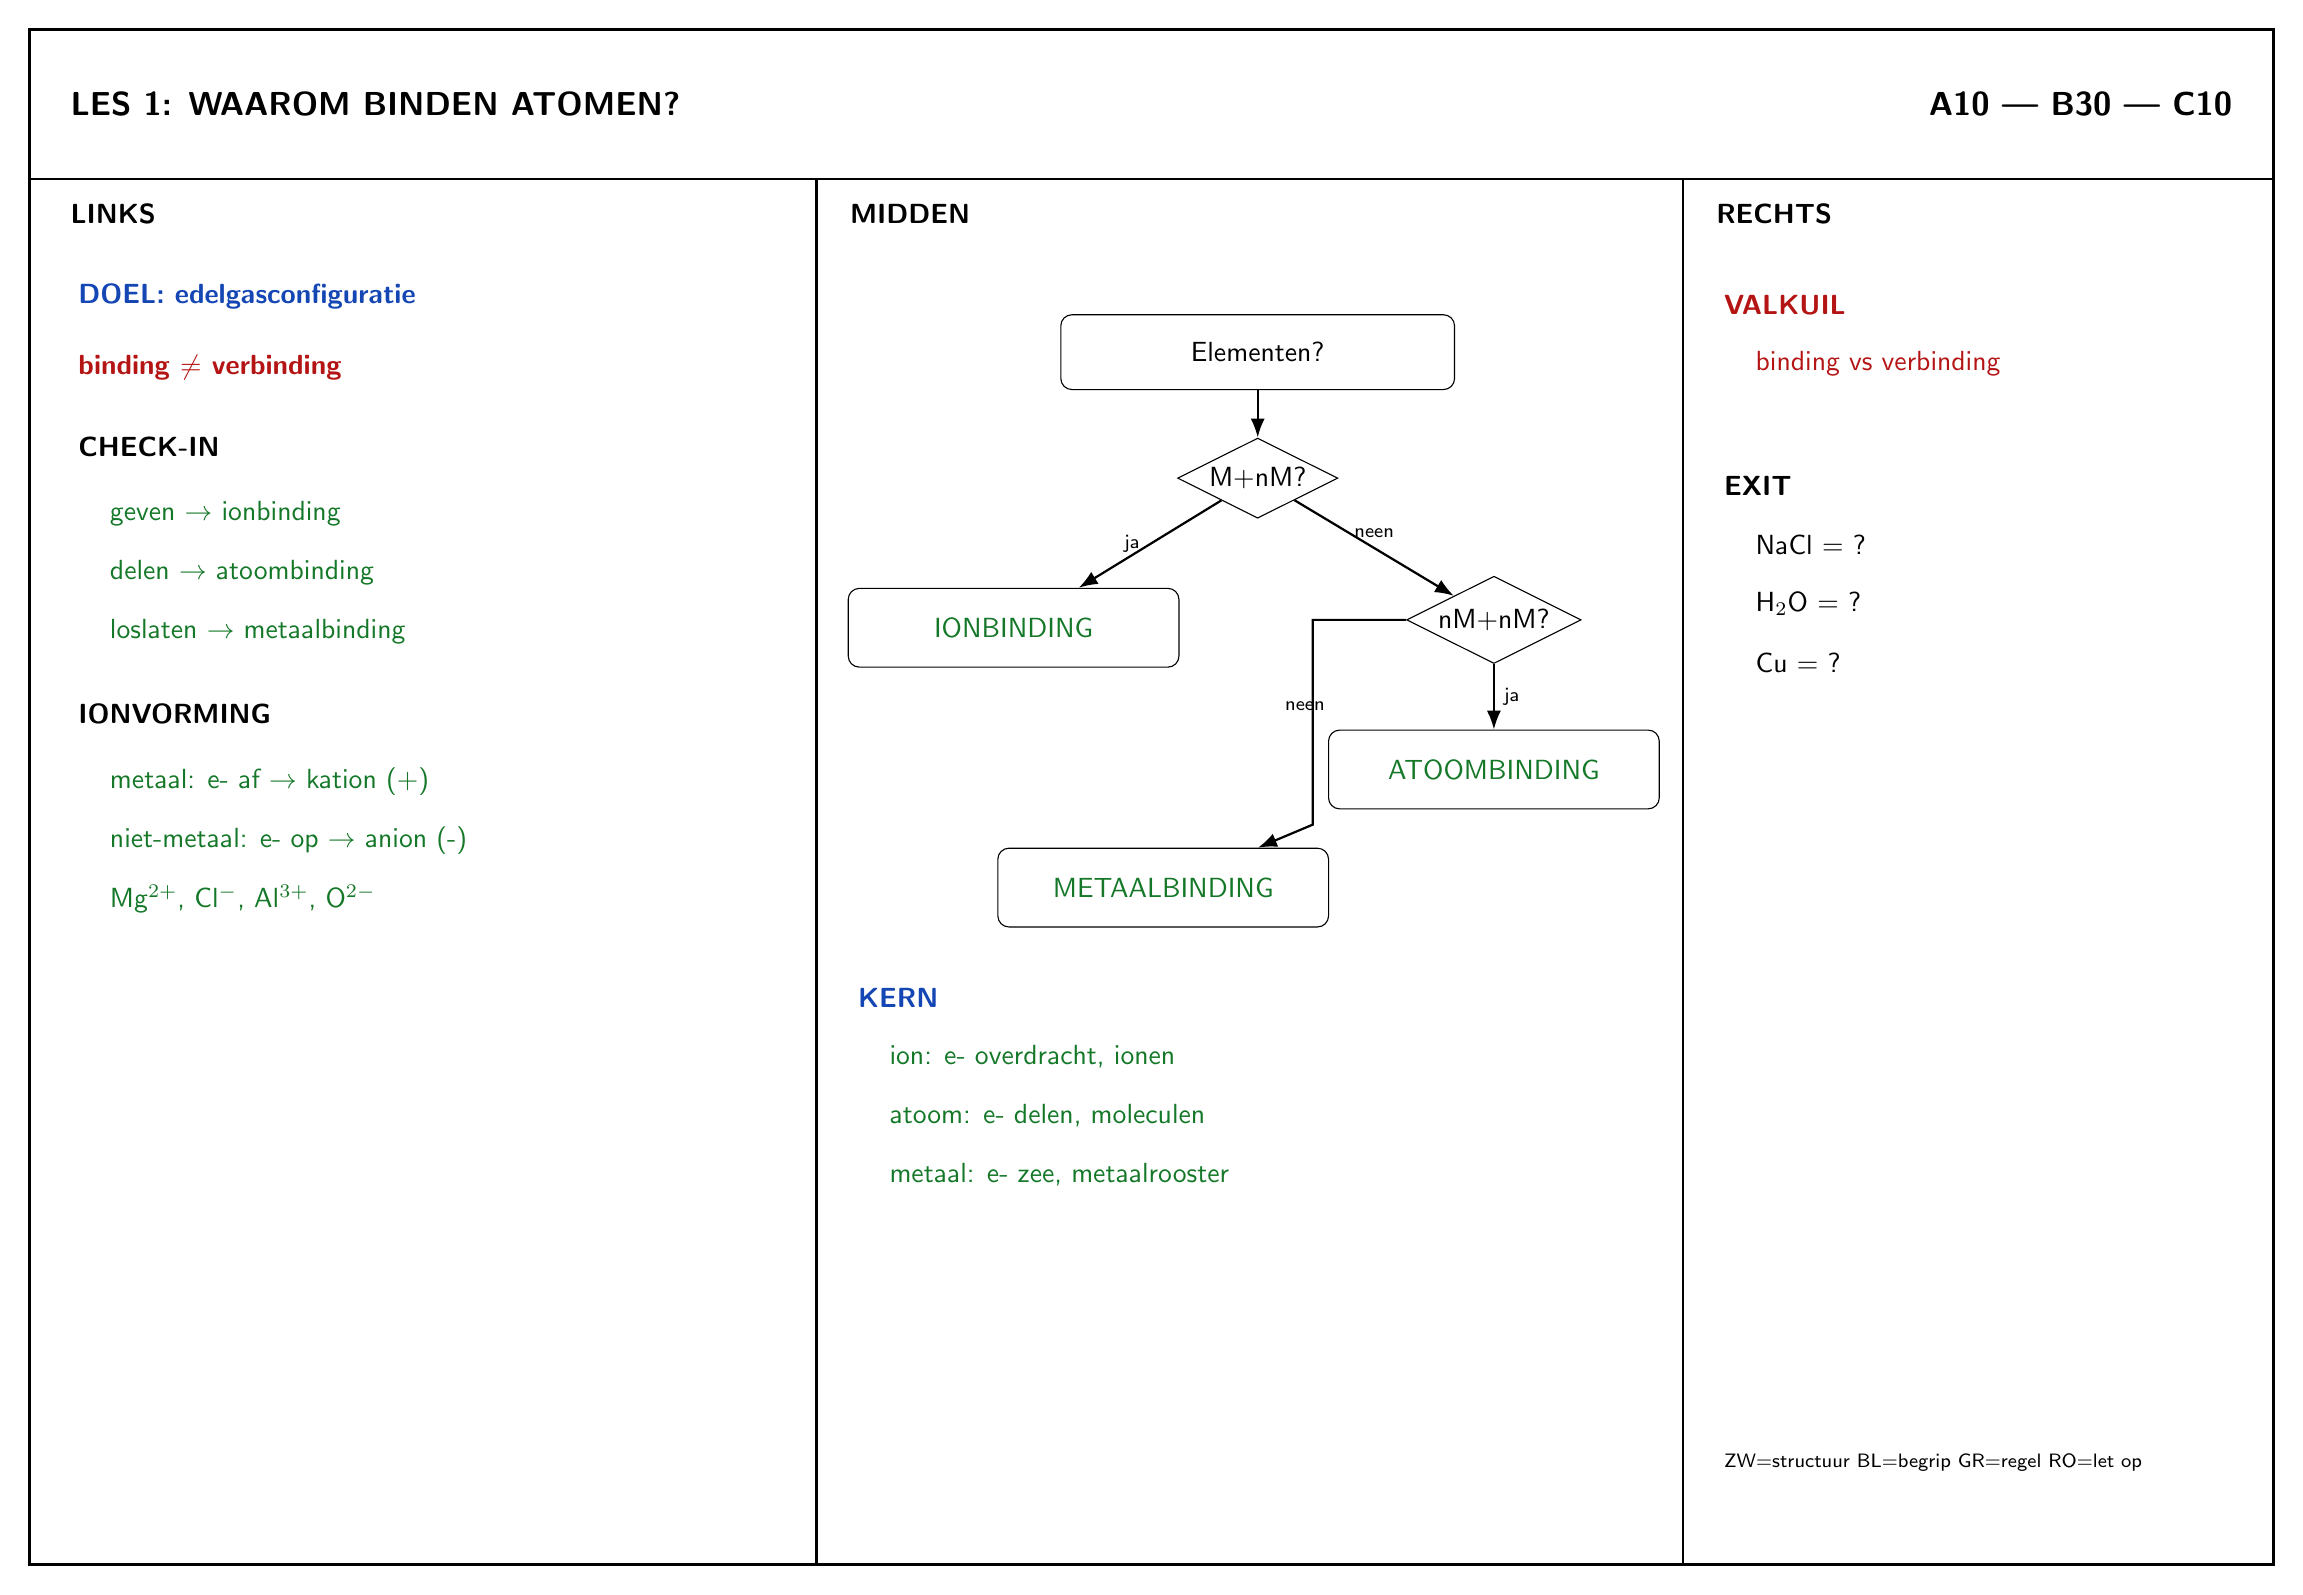
\begin{tikzpicture}[x=1cm,y=1cm]
  % outer board
  \draw[line width=1.2pt] (0,0) rectangle (28.5,19.5);

  % top bar
  \draw[line width=0.9pt] (0,17.6) -- (28.5,17.6);
  \node[anchor=west,font=\bfseries\large] at (0.4,18.55) {\ZW{LES 1: WAAROM BINDEN ATOMEN?}};
  \node[anchor=east,font=\bfseries\large] at (28.1,18.55) {\ZW{A10 | B30 | C10}};

  % vertical columns
  \draw[line width=0.9pt] (10.0,0) -- (10.0,17.6);
  \draw[line width=0.9pt] (21.0,0) -- (21.0,17.6);

  % column titles
  \node[anchor=west,font=\bfseries] at (0.4,17.15) {\ZW{LINKS}};
  \node[anchor=west,font=\bfseries] at (10.3,17.15) {\ZW{MIDDEN}};
  \node[anchor=west,font=\bfseries] at (21.3,17.15) {\ZW{RECHTS}};

  % left content
  \node[anchor=west,font=\bfseries] at (0.5,16.1) {\BL{DOEL: edelgasconfiguratie}};
  \node[anchor=west,font=\bfseries] at (0.5,15.2) {\RO{binding $\neq$ verbinding}};
  \node[anchor=west,font=\bfseries] at (0.5,14.2) {\ZW{CHECK-IN}};
  \node[anchor=west] at (0.9,13.35) {\GR{geven $\rightarrow$ ionbinding}};
  \node[anchor=west] at (0.9,12.6) {\GR{delen $\rightarrow$ atoombinding}};
  \node[anchor=west] at (0.9,11.85) {\GR{loslaten $\rightarrow$ metaalbinding}};

  \node[anchor=west,font=\bfseries] at (0.5,10.8) {\ZW{IONVORMING}};
  \node[anchor=west] at (0.9,9.95) {\GR{metaal: e- af $\rightarrow$ kation (+)}};
  \node[anchor=west] at (0.9,9.2) {\GR{niet-metaal: e- op $\rightarrow$ anion (-)}};
  \node[anchor=west] at (0.9,8.45) {\GR{Mg$^{2+}$, Cl$^{-}$, Al$^{3+}$, O$^{2-}$}};

  % middle content - decision flow
  \node[draw,rounded corners,minimum width=5.0cm,minimum height=0.95cm,align=center] (s1) at (15.6,15.4) {\ZW{Elementen?}};
  \node[draw,diamond,aspect=2.0,inner sep=1.2pt,align=center] (q1) at (15.6,13.8) {\ZW{M+nM?}};
  \node[draw,rounded corners,minimum width=4.2cm,minimum height=1.0cm,align=center] (ion) at (12.5,11.9) {\GR{IONBINDING}};
  \node[draw,diamond,aspect=2.0,inner sep=1.2pt,align=center] (q2) at (18.6,12.0) {\ZW{nM+nM?}};
  \node[draw,rounded corners,minimum width=4.2cm,minimum height=1.0cm,align=center] (atoom) at (18.6,10.1) {\GR{ATOOMBINDING}};
  \node[draw,rounded corners,minimum width=4.2cm,minimum height=1.0cm,align=center] (metaal) at (14.4,8.6) {\GR{METAALBINDING}};

  \draw[-{Latex[length=2.4mm]},line width=0.8pt] (s1) -- (q1);
  \draw[-{Latex[length=2.4mm]},line width=0.8pt] (q1) -- node[left,font=\scriptsize]{\ZW{ja}} (ion);
  \draw[-{Latex[length=2.4mm]},line width=0.8pt] (q1) -- node[above,font=\scriptsize]{\ZW{neen}} (q2);
  \draw[-{Latex[length=2.4mm]},line width=0.8pt] (q2) -- node[right,font=\scriptsize]{\ZW{ja}} (atoom);
  \draw[-{Latex[length=2.4mm]},line width=0.8pt] (q2) -- ++(-2.3,0) -- ++(0,-2.6) -- (metaal);
  \node[font=\scriptsize] at (16.2,10.9) {\ZW{neen}};

  \node[anchor=west,font=\bfseries] at (10.4,7.2) {\BL{KERN}};
  \node[anchor=west] at (10.8,6.45) {\GR{ion: e- overdracht, ionen}};
  \node[anchor=west] at (10.8,5.7) {\GR{atoom: e- delen, moleculen}};
  \node[anchor=west] at (10.8,4.95) {\GR{metaal: e- zee, metaalrooster}};

  % right content
  \node[anchor=west,font=\bfseries] at (21.4,16.0) {\RO{VALKUIL}};
  \node[anchor=west] at (21.8,15.25) {\RO{binding vs verbinding}};

  \node[anchor=west,font=\bfseries] at (21.4,13.7) {\ZW{EXIT}};
  \node[anchor=west] at (21.8,12.95) {\ZW{NaCl = ?}};
  \node[anchor=west] at (21.8,12.2) {\ZW{H$_2$O = ?}};
  \node[anchor=west] at (21.8,11.45) {\ZW{Cu = ?}};

  % marker legend on board edge (minimal)
  \node[anchor=west,font=\scriptsize] at (21.4,1.3) {\ZW{ZW=structuur  BL=begrip  GR=regel  RO=let op}};
\end{tikzpicture}

\newpage

% ========================= LES 2 =========================
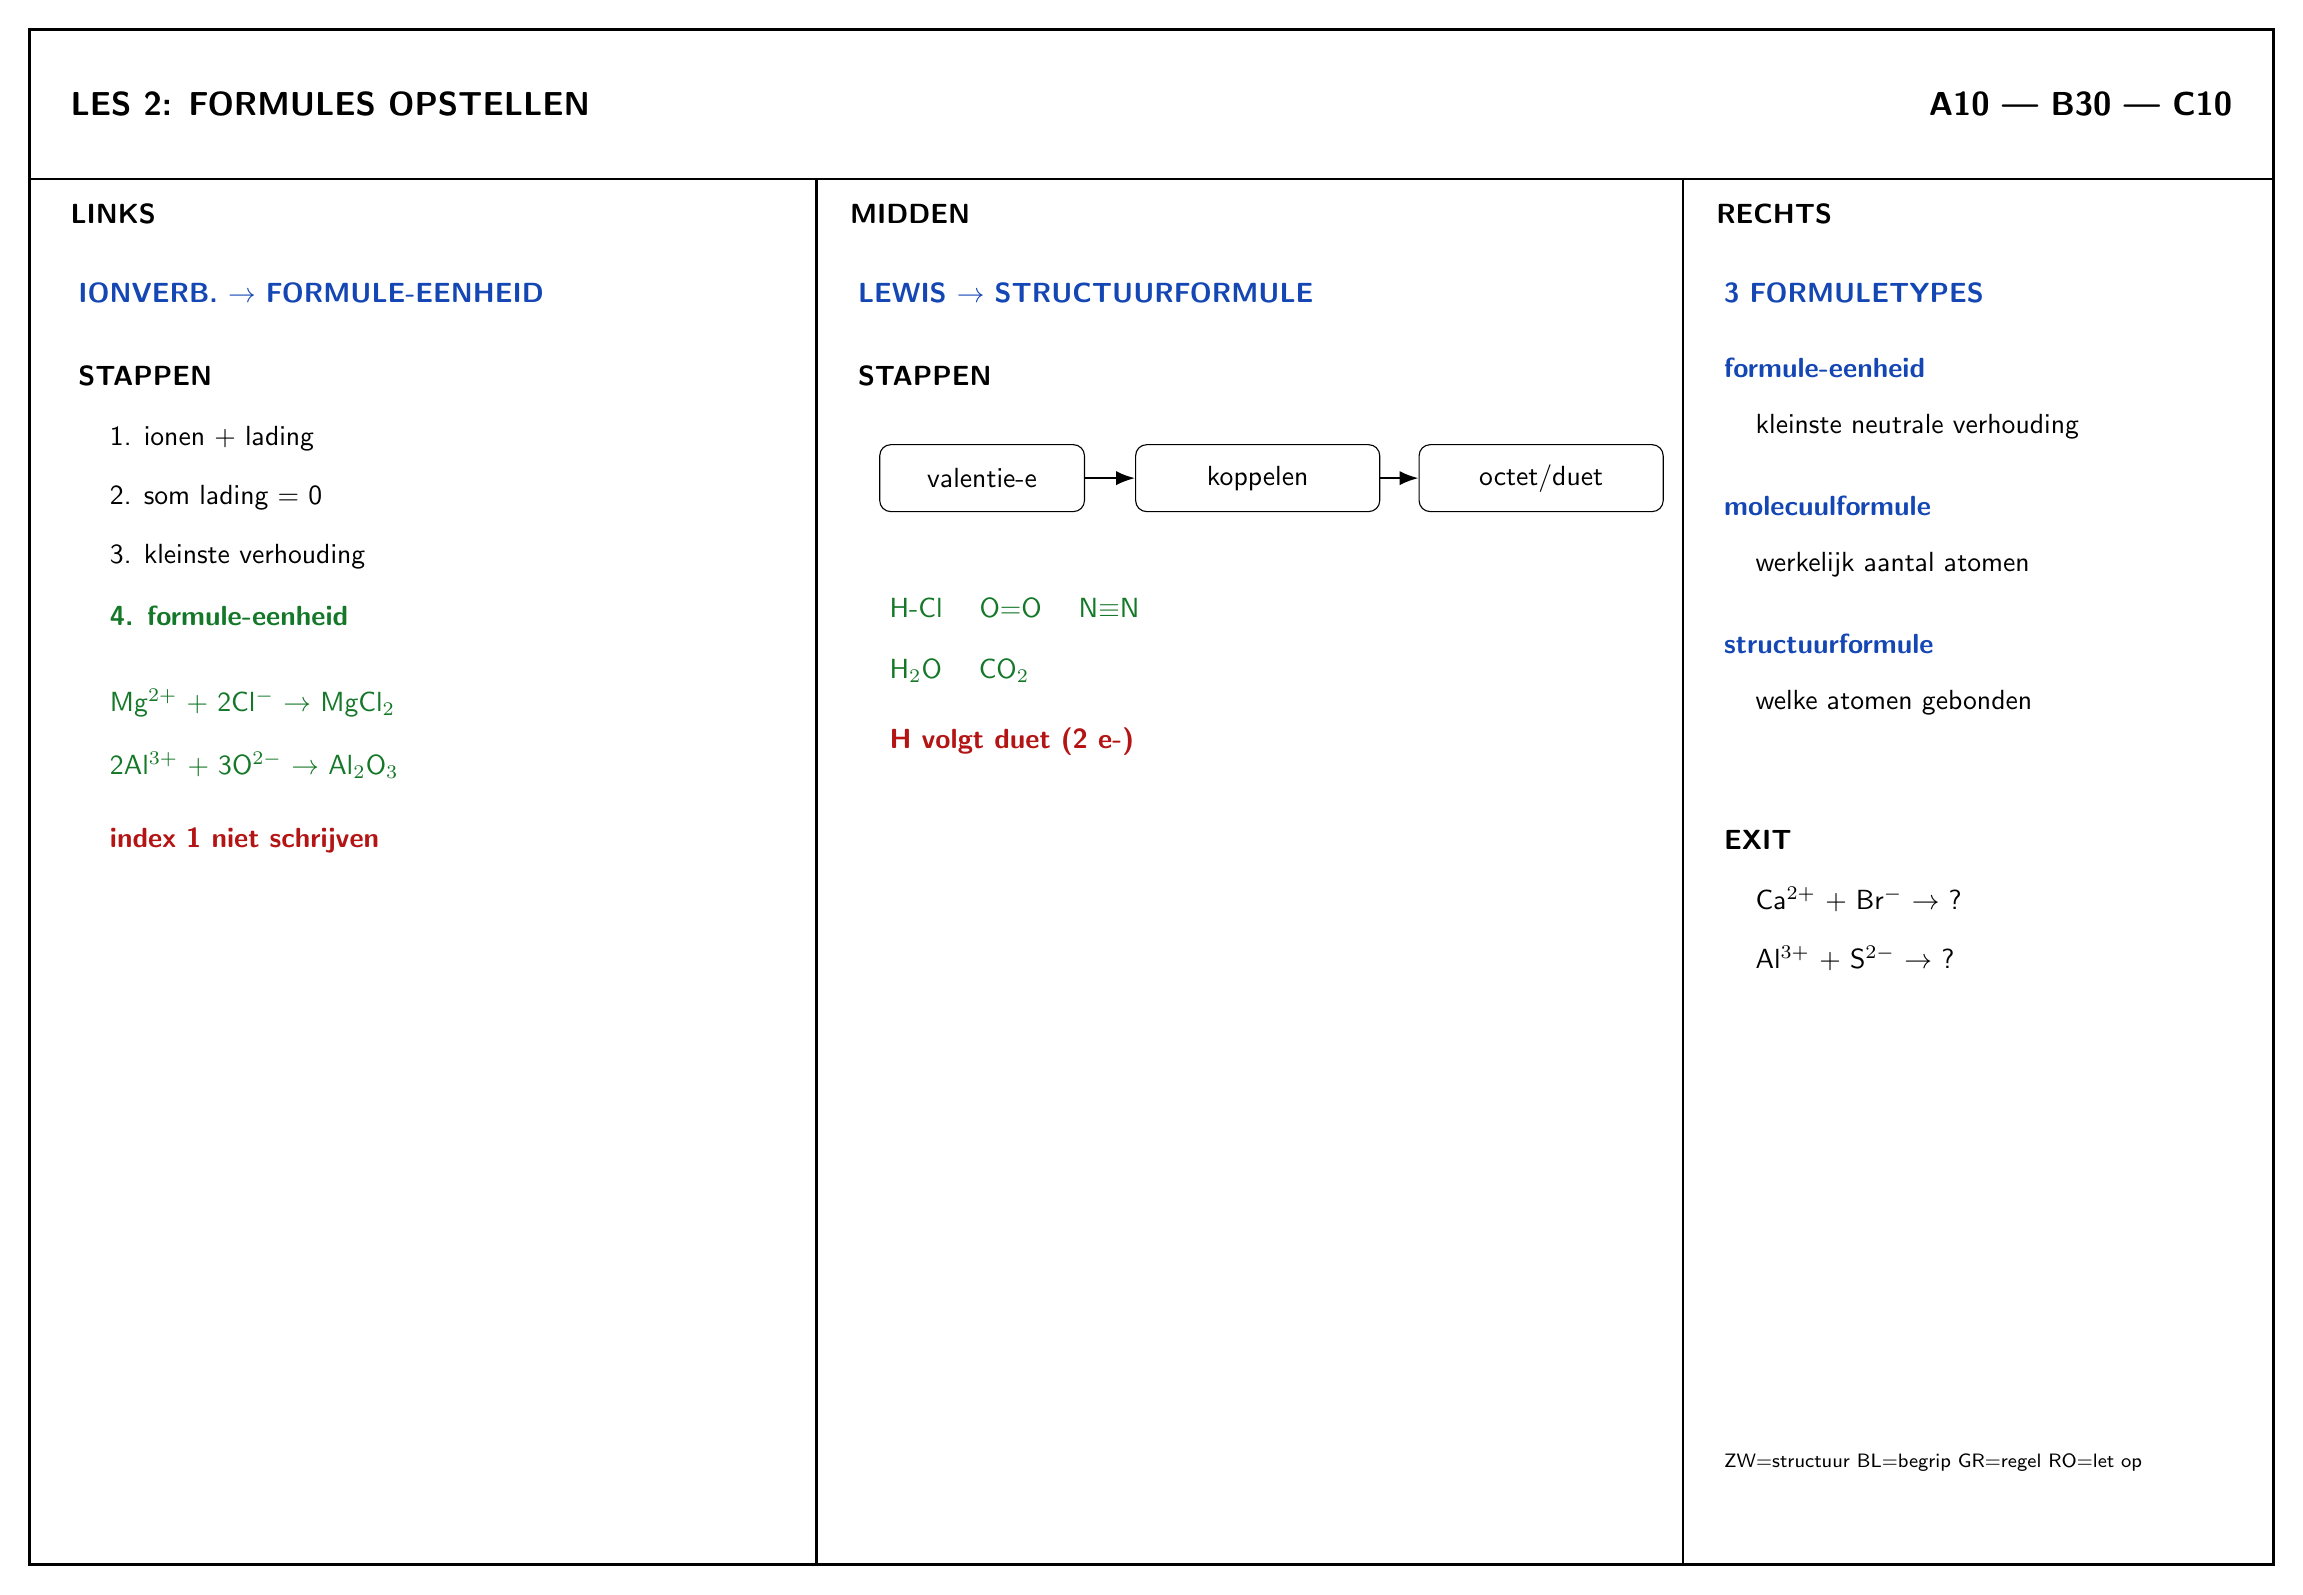
\begin{tikzpicture}[x=1cm,y=1cm]
  \draw[line width=1.2pt] (0,0) rectangle (28.5,19.5);
  \draw[line width=0.9pt] (0,17.6) -- (28.5,17.6);
  \node[anchor=west,font=\bfseries\large] at (0.4,18.55) {\ZW{LES 2: FORMULES OPSTELLEN}};
  \node[anchor=east,font=\bfseries\large] at (28.1,18.55) {\ZW{A10 | B30 | C10}};

  \draw[line width=0.9pt] (10.0,0) -- (10.0,17.6);
  \draw[line width=0.9pt] (21.0,0) -- (21.0,17.6);
  \node[anchor=west,font=\bfseries] at (0.4,17.15) {\ZW{LINKS}};
  \node[anchor=west,font=\bfseries] at (10.3,17.15) {\ZW{MIDDEN}};
  \node[anchor=west,font=\bfseries] at (21.3,17.15) {\ZW{RECHTS}};

  % left
  \node[anchor=west,font=\bfseries] at (0.5,16.15) {\BL{IONVERB. $\rightarrow$ FORMULE-EENHEID}};
  \node[anchor=west,font=\bfseries] at (0.5,15.1) {\ZW{STAPPEN}};
  \node[anchor=west] at (0.9,14.3) {\ZW{1. ionen + lading}};
  \node[anchor=west] at (0.9,13.55) {\ZW{2. som lading = 0}};
  \node[anchor=west] at (0.9,12.8) {\ZW{3. kleinste verhouding}};
  \node[anchor=west,font=\bfseries] at (0.9,12.05) {\GR{4. formule-eenheid}};
  \node[anchor=west] at (0.9,10.95) {\GR{Mg$^{2+}$ + 2Cl$^{-}$ $\rightarrow$ MgCl$_2$}};
  \node[anchor=west] at (0.9,10.15) {\GR{2Al$^{3+}$ + 3O$^{2-}$ $\rightarrow$ Al$_2$O$_3$}};
  \node[anchor=west,font=\bfseries] at (0.9,9.2) {\RO{index 1 niet schrijven}};

  % middle
  \node[anchor=west,font=\bfseries] at (10.4,16.15) {\BL{LEWIS $\rightarrow$ STRUCTUURFORMULE}};
  \node[anchor=west,font=\bfseries] at (10.4,15.1) {\ZW{STAPPEN}};

  \node[draw,rounded corners,minimum width=2.6cm,minimum height=0.85cm] (l1) at (12.1,13.8) {\ZW{valentie-e}};
  \node[draw,rounded corners,minimum width=3.1cm,minimum height=0.85cm] (l2) at (15.6,13.8) {\ZW{koppelen}};
  \node[draw,rounded corners,minimum width=3.1cm,minimum height=0.85cm] (l3) at (19.2,13.8) {\ZW{octet/duet}};
  \draw[-{Latex[length=2.4mm]},line width=0.8pt] (l1) -- (l2);
  \draw[-{Latex[length=2.4mm]},line width=0.8pt] (l2) -- (l3);

  \node[anchor=west] at (10.8,12.15) {\GR{H-Cl \quad O=O \quad N$\equiv$N}};
  \node[anchor=west] at (10.8,11.35) {\GR{H$_2$O \quad CO$_2$}};
  \node[anchor=west,font=\bfseries] at (10.8,10.45) {\RO{H volgt duet (2 e-)}};

  % right
  \node[anchor=west,font=\bfseries] at (21.4,16.15) {\BL{3 FORMULETYPES}};
  \node[anchor=west,font=\bfseries] at (21.4,15.2) {\BL{formule-eenheid}};
  \node[anchor=west] at (21.8,14.45) {\ZW{kleinste neutrale verhouding}};
  \node[anchor=west,font=\bfseries] at (21.4,13.45) {\BL{molecuulformule}};
  \node[anchor=west] at (21.8,12.7) {\ZW{werkelijk aantal atomen}};
  \node[anchor=west,font=\bfseries] at (21.4,11.7) {\BL{structuurformule}};
  \node[anchor=west] at (21.8,10.95) {\ZW{welke atomen gebonden}};

  \node[anchor=west,font=\bfseries] at (21.4,9.2) {\ZW{EXIT}};
  \node[anchor=west] at (21.8,8.45) {\ZW{Ca$^{2+}$ + Br$^{-}$ $\rightarrow$ ?}};
  \node[anchor=west] at (21.8,7.7) {\ZW{Al$^{3+}$ + S$^{2-}$ $\rightarrow$ ?}};

  \node[anchor=west,font=\scriptsize] at (21.4,1.3) {\ZW{ZW=structuur  BL=begrip  GR=regel  RO=let op}};
\end{tikzpicture}

\newpage

% ========================= LES 3 =========================
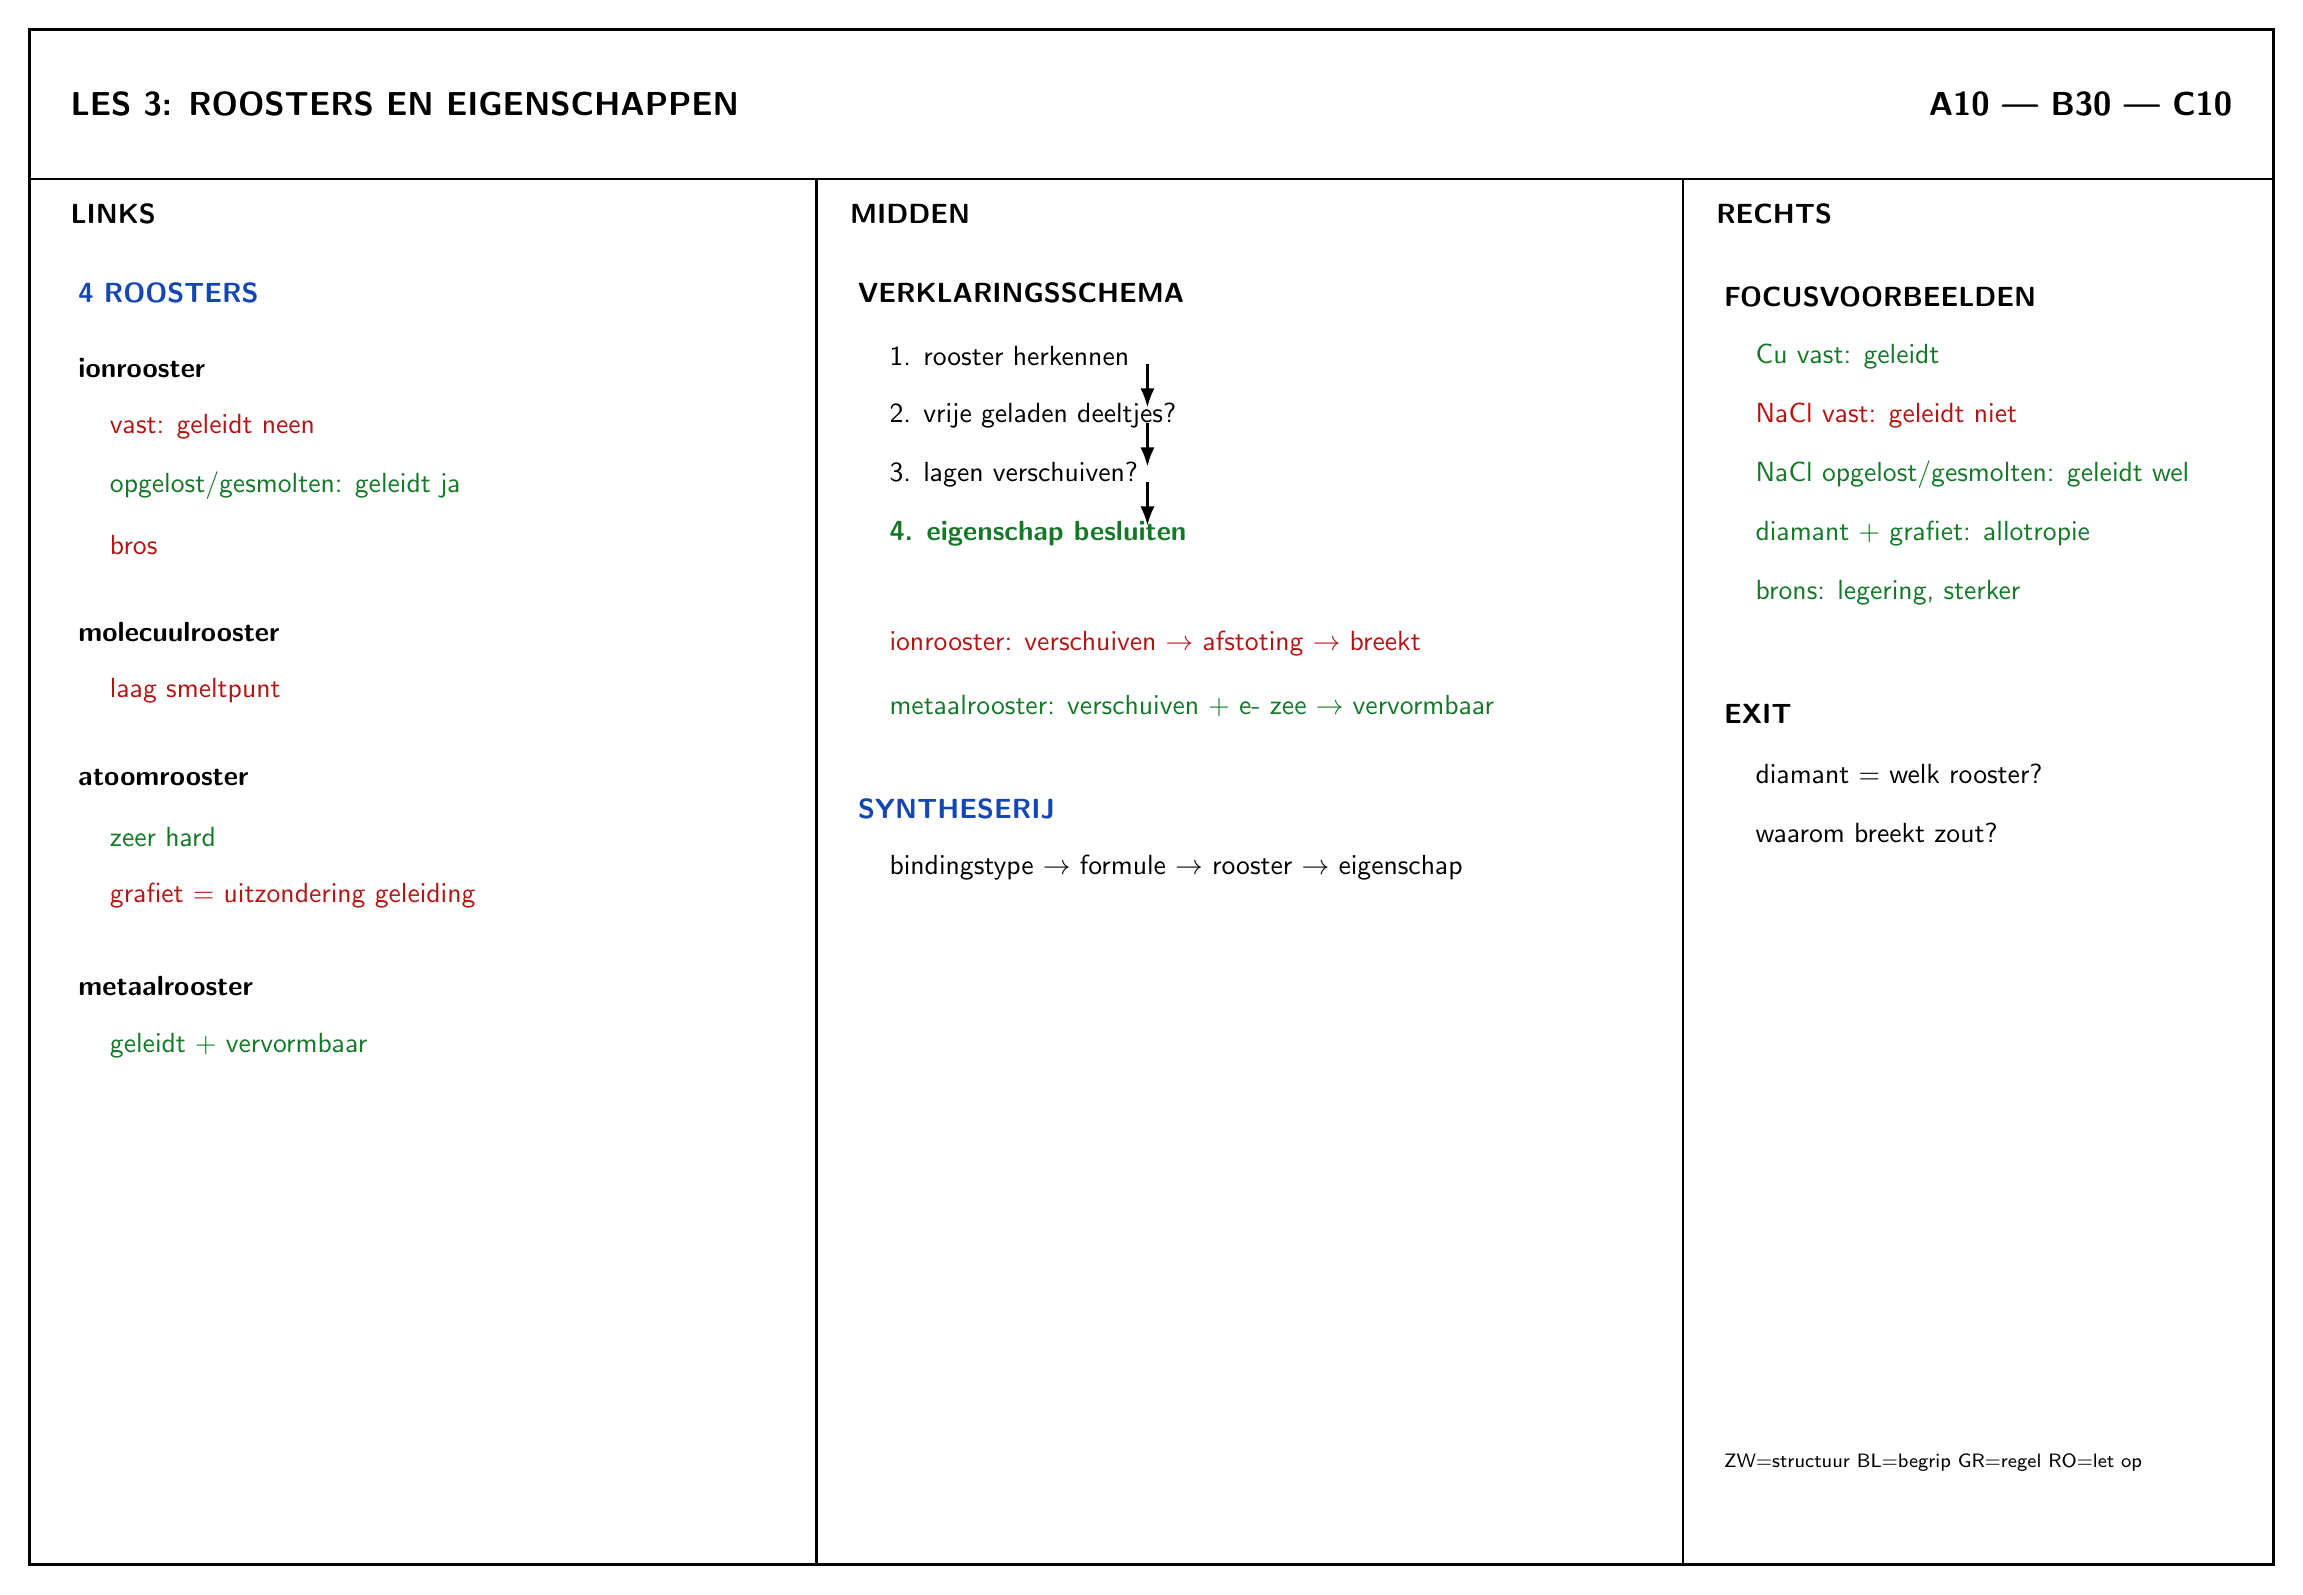
\begin{tikzpicture}[x=1cm,y=1cm]
  \draw[line width=1.2pt] (0,0) rectangle (28.5,19.5);
  \draw[line width=0.9pt] (0,17.6) -- (28.5,17.6);
  \node[anchor=west,font=\bfseries\large] at (0.4,18.55) {\ZW{LES 3: ROOSTERS EN EIGENSCHAPPEN}};
  \node[anchor=east,font=\bfseries\large] at (28.1,18.55) {\ZW{A10 | B30 | C10}};

  \draw[line width=0.9pt] (10.0,0) -- (10.0,17.6);
  \draw[line width=0.9pt] (21.0,0) -- (21.0,17.6);
  \node[anchor=west,font=\bfseries] at (0.4,17.15) {\ZW{LINKS}};
  \node[anchor=west,font=\bfseries] at (10.3,17.15) {\ZW{MIDDEN}};
  \node[anchor=west,font=\bfseries] at (21.3,17.15) {\ZW{RECHTS}};

  % left
  \node[anchor=west,font=\bfseries] at (0.5,16.15) {\BL{4 ROOSTERS}};
  \node[anchor=west,font=\bfseries] at (0.5,15.2) {\ZW{ionrooster}};
  \node[anchor=west] at (0.9,14.45) {\RO{vast: geleidt neen}};
  \node[anchor=west] at (0.9,13.7) {\GR{opgelost/gesmolten: geleidt ja}};
  \node[anchor=west] at (0.9,12.95) {\RO{bros}};

  \node[anchor=west,font=\bfseries] at (0.5,11.85) {\ZW{molecuulrooster}};
  \node[anchor=west] at (0.9,11.1) {\RO{laag smeltpunt}};

  \node[anchor=west,font=\bfseries] at (0.5,10.0) {\ZW{atoomrooster}};
  \node[anchor=west] at (0.9,9.25) {\GR{zeer hard}};
  \node[anchor=west] at (0.9,8.5) {\RO{grafiet = uitzondering geleiding}};

  \node[anchor=west,font=\bfseries] at (0.5,7.35) {\ZW{metaalrooster}};
  \node[anchor=west] at (0.9,6.6) {\GR{geleidt + vervormbaar}};

  % middle
  \node[anchor=west,font=\bfseries] at (10.4,16.15) {\ZW{VERKLARINGSSCHEMA}};
  \node[anchor=west] at (10.8,15.35) {\ZW{1. rooster herkennen}};
  \node[anchor=west] at (10.8,14.6) {\ZW{2. vrije geladen deeltjes?}};
  \node[anchor=west] at (10.8,13.85) {\ZW{3. lagen verschuiven?}};
  \node[anchor=west,font=\bfseries] at (10.8,13.1) {\GR{4. eigenschap besluiten}};

  \draw[-{Latex[length=2.4mm]},line width=0.8pt] (14.2,15.25) -- (14.2,14.7);
  \draw[-{Latex[length=2.4mm]},line width=0.8pt] (14.2,14.5) -- (14.2,13.95);
  \draw[-{Latex[length=2.4mm]},line width=0.8pt] (14.2,13.75) -- (14.2,13.2);

  \node[anchor=west] at (10.8,11.7) {\RO{ionrooster: verschuiven $\rightarrow$ afstoting $\rightarrow$ breekt}};
  \node[anchor=west] at (10.8,10.9) {\GR{metaalrooster: verschuiven + e- zee $\rightarrow$ vervormbaar}};

  \node[anchor=west,font=\bfseries] at (10.4,9.6) {\BL{SYNTHESERIJ}};
  \node[anchor=west] at (10.8,8.85) {\ZW{bindingstype $\rightarrow$ formule $\rightarrow$ rooster $\rightarrow$ eigenschap}};

  % right
  \node[anchor=west,font=\bfseries] at (21.4,16.1) {\ZW{FOCUSVOORBEELDEN}};
  \node[anchor=west] at (21.8,15.35) {\GR{Cu vast: geleidt}};
  \node[anchor=west] at (21.8,14.6) {\RO{NaCl vast: geleidt niet}};
  \node[anchor=west] at (21.8,13.85) {\GR{NaCl opgelost/gesmolten: geleidt wel}};
  \node[anchor=west] at (21.8,13.1) {\GR{diamant + grafiet: allotropie}};
  \node[anchor=west] at (21.8,12.35) {\GR{brons: legering, sterker}};

  \node[anchor=west,font=\bfseries] at (21.4,10.8) {\ZW{EXIT}};
  \node[anchor=west] at (21.8,10.05) {\ZW{diamant = welk rooster?}};
  \node[anchor=west] at (21.8,9.3) {\ZW{waarom breekt zout?}};

  \node[anchor=west,font=\scriptsize] at (21.4,1.3) {\ZW{ZW=structuur  BL=begrip  GR=regel  RO=let op}};
\end{tikzpicture}

\end{document}
